\documentclass{beamer}\usepackage[]{graphicx}\usepackage[]{color}
%% maxwidth is the original width if it is less than linewidth
%% otherwise use linewidth (to make sure the graphics do not exceed the margin)
\makeatletter
\def\maxwidth{ %
  \ifdim\Gin@nat@width>\linewidth
    \linewidth
  \else
    \Gin@nat@width
  \fi
}
\makeatother

\definecolor{fgcolor}{rgb}{0.345, 0.345, 0.345}
\newcommand{\hlnum}[1]{\textcolor[rgb]{0.686,0.059,0.569}{#1}}%
\newcommand{\hlstr}[1]{\textcolor[rgb]{0.192,0.494,0.8}{#1}}%
\newcommand{\hlcom}[1]{\textcolor[rgb]{0.678,0.584,0.686}{\textit{#1}}}%
\newcommand{\hlopt}[1]{\textcolor[rgb]{0,0,0}{#1}}%
\newcommand{\hlstd}[1]{\textcolor[rgb]{0.345,0.345,0.345}{#1}}%
\newcommand{\hlkwa}[1]{\textcolor[rgb]{0.161,0.373,0.58}{\textbf{#1}}}%
\newcommand{\hlkwb}[1]{\textcolor[rgb]{0.69,0.353,0.396}{#1}}%
\newcommand{\hlkwc}[1]{\textcolor[rgb]{0.333,0.667,0.333}{#1}}%
\newcommand{\hlkwd}[1]{\textcolor[rgb]{0.737,0.353,0.396}{\textbf{#1}}}%

\usepackage{framed}
\makeatletter
\newenvironment{kframe}{%
 \def\at@end@of@kframe{}%
 \ifinner\ifhmode%
  \def\at@end@of@kframe{\end{minipage}}%
  \begin{minipage}{\columnwidth}%
 \fi\fi%
 \def\FrameCommand##1{\hskip\@totalleftmargin \hskip-\fboxsep
 \colorbox{shadecolor}{##1}\hskip-\fboxsep
     % There is no \\@totalrightmargin, so:
     \hskip-\linewidth \hskip-\@totalleftmargin \hskip\columnwidth}%
 \MakeFramed {\advance\hsize-\width
   \@totalleftmargin\z@ \linewidth\hsize
   \@setminipage}}%
 {\par\unskip\endMakeFramed%
 \at@end@of@kframe}
\makeatother

\definecolor{shadecolor}{rgb}{.97, .97, .97}
\definecolor{messagecolor}{rgb}{0, 0, 0}
\definecolor{warningcolor}{rgb}{1, 0, 1}
\definecolor{errorcolor}{rgb}{1, 0, 0}
\newenvironment{knitrout}{}{} % an empty environment to be redefined in TeX

\usepackage{alltt}
\usefonttheme[onlymath]{serif}

\usepackage[english,portuguese]{babel}
\usepackage{graphicx}
\usepackage{ulem} % Para texto em strikeout
\usepackage{amsmath}
\usepackage{amssymb}
\usepackage{hyperref}

\usepackage{tikz}
\usepackage{tikz-qtree}
\tikzset{edge from parent/.style={draw,very thick}}

\usetheme{m}

\title{Aula 1: Estatística e Probabilidade}
\subtitle{Análise Quantitativa de Dados Ambientais}
\author{\textbf{Thiago S. F. Silva} - tsfsilva@rc.unesp.br}
\institute{Programa de Pós Graduação em Geografia - IGCE/UNESP}
\date{\today}
\IfFileExists{upquote.sty}{\usepackage{upquote}}{}
\begin{document}




%===============================================================================%
\begin{frame}[plain] % plain avoids a badbox error from page number in title page
  \titlepage
\end{frame}

\begin{frame}{Outline}
  \tableofcontents
\end{frame}
%===============================================================================%


\section{Visão Geral do Curso}


%===============================================================================%
\begin{frame}{Funcionamento do Curso} 

  O curso se divide em:
  
  \begin{itemize}
    
    \item{\sout{Blá, blá, blá, blá}  \hspace{7.5mm}\textbf{Aulas Teóricas}}
    \item{\sout{Brigando com o R}  \hspace{4mm}\textbf{Práticas e Exercícios}}
    \item{\sout{Zzzzzzzzzzzzzzz} \hspace{9.5mm}\textbf{Discussões de artigos}}
  
  \end{itemize}
  
  \vfill
  
  Avaliação:
  
  \begin{itemize}
  
  \item{\textbf{Exercícios:} scripts de análise derivados das aulas práticas}
  \item{\textbf{Bootcamp:} maratona de análise de um mini-projeto, em sala}
  \item{\textbf{Seus próprios dados ou dados pré-adquiridos, à sua escolha}}
  
  \end{itemize}
  
  
\end{frame} 
%===============================================================================%

% %===============================================================================%
% \begin{frame}{Funcionamento do Curso} 
% 
%   Todo o material estará disponível no Dropbox:
%   
% \scriptsize{\url{https://www.dropbox.com/sh/9u79oybayyi86zw/AAAW_8GTZShFnA8BrzFbe-LDa?dl=0}}
%   
%   \begin{itemize}
%     
%     \item Slides
%     \item Artigos
%     \item Livros
%     \item Exercícios
%     \item Dados
%       
%   \end{itemize}
%       
% \end{frame} 
% %===============================================================================%

%===============================================================================%
\begin{frame}{Sim, nós temos um plano} 

\begin{small}

  \begin{itemize}
    
    \item{2015-08-24: Introdução, Probabilidades}
    
    \item{2015-08-25: Distribuições de Probabilidade}
    
    \item{2015-08-26: Testes de Hipóteses}
    
    \item{2015-08-27: Erros Tipo I e Tipo II}
    
    \item{2015-08-28: Organização de Dados, Análise Exploratória e Gráfica}
    
    \item{2015-08-31: Modelos Lineares Gerais: Regressão Simples e Multivariada}
    
    \item{2015-09-01: Modelos Lineares Gerais: ANOVA e ANCOVA}
    
    \item{2015-09-02: Modelos Lineares Gerais: Diagnóstico e Remediação}
            
    \item{2015-09-03: Bootcamp de Análise de dados}
    
  \end{itemize}

\alert{Plano sujeito à mudanças, sempre.}

\end{small}

\end{frame} 
%===============================================================================%

%===============================================================================%
\begin{frame}{Apresentações}

  \begin{itemize}
    \item{\textbf{Thiago Sanna Freire Silva}}
    \item{Departamento de Geografia - IGCE/UNESP}
    \item{tsfsilva@rc.unesp.br - (19) 3526-9208}
  \end{itemize}
  
  \vfill
  
  \begin{itemize}
    \item{Biólogo (UFRN)}
    \item{Mestre em Sensoriamento Remoto (INPE)}
    \item{Doutor em Geografia (UVic - Canadá)}
  \end{itemize}
  
  \vfill
  
  \begin{itemize}
      \item{Funcionamento de ecossistemas e mudanças climáticas}
      \item{Dinâmica espaço-temporal de paisagens}
      \item{Interface entre Ecologia, Computação e Geociências}
      
  \end{itemize}
  
\end{frame}
%===============================================================================%

%===============================================================================%
\begin{frame}{Apresentações}

\vfill

\center{\textbf{\huge{Vocês?}}}

\vfill

\end{frame}
%===============================================================================%

\section{O que é Estatística?}

%===============================================================================%
\begin{frame}{O que é Estatística?}

O que é Estatística? \pause

\vfill

  O que a Estatística \textbf{não} é: 

  \begin{itemize}
  
    \item{Uma ciência exata}
    
    \item{Um método único e infalível}
    
    \item{Um sistema automático de decisão}
    
    \item{Uma solução para todos os problemas científicos}
    
    \item{A salvação para uma pesquisa ruim}
    
   \end{itemize}
    
\scriptsize{``To consult the statistician after an experiment is finished is often merely to ask him to conduct a post mortem examination. He can perhaps say what the experiment died of''. - \emph{Sir} Ronald Fisher.}

\end{frame}
%===============================================================================%


%===============================================================================%
\begin{frame}{O que é Estatística?}

  Matemática vs. Estatística: é a mesma coisa?
  \pause
  
  \vfill
  
  Pra que serve a Estatística? \pause
  \vfill

  Propósito da Estatística: estimar e quantificar \textbf{incertezas}
  
  \vfill
  
  Incertezas = \textbf{probabilidades}

\end{frame}
%===============================================================================%


%===============================================================================%
\begin{frame}{O que é Estatística?}

  Como podemos quantificar incertezas acerca de alguma coisa? \pause
  
  \vfill
  
  \begin{itemize}
  
    \item{Observações...}
    
    \vfill
    
    \item{Repetições...}
    
    \vfill
    
    \item{Experimentos...} 
  
  \end{itemize}
    
\end{frame}
%===============================================================================%

%===============================================================================%
\begin{frame}{O que é Estatística?}

  Por que queremos quantificar incertezas acerca de alguma coisa? \pause
  
  \vfill
  
  \begin{itemize}
  
    \item{Decisão...}
    
    \vfill
    
    \item{Explicação...}
    
    \vfill
    
    \item{Previsão...} 
  
  \end{itemize}
    
\end{frame}
%===============================================================================%

%===============================================================================%
\begin{frame}{Exemplos}

\begin{small}

 \begin{itemize}
  
      \item{Um reservatório tem 60\% de chance de eliminar o habitat de uma espécie. Mas há 75\% de chance de que o investimento dos royalties vá garantir a preservação de 500km$^2$ de floresta primária no entorno do reservatório. Será que devo autorizar ou vetar a construção desse reservatório?}
    
    \vfill
    
      \item{Qual a contribuição relativa do regime hidrológico, quantidade de nutrientes, e turbidez da água no crescimento de plantas aquáticas na Amazônia?}
  
  \vfill
  
    \item{Com que grau de certeza posso afirmar que a diversidade irá aumentar em 1.5 vezes quando a disponibilidade de nutrientes aumenta em 0.7 vezes?}
  
  \end{itemize}
  
\end{small}

\end{frame}
%===============================================================================%


\section{Modelagem Estatística}


%===============================================================================%
\begin{frame}{Modelos}
\begin{columns}[c]
\column{3in}
\huge{O que é um \textbf{modelo}?}

\column{1.5in}
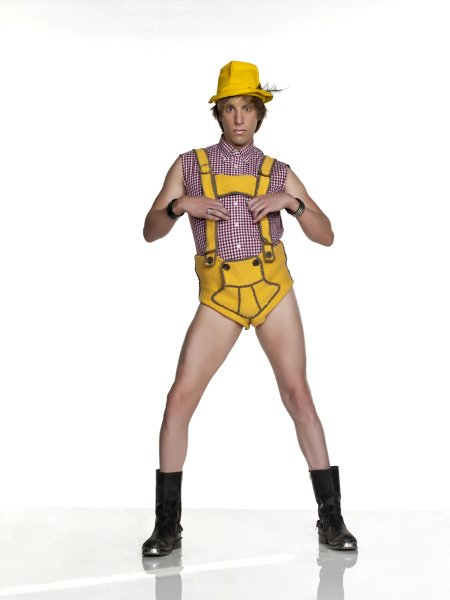
\includegraphics[width=2in, trim= 100 0 0 50, clip]{C:/Users/thiago/OneDrive/UNESP/Pos_graduacao/Eco/2015/Estatistica_2015/Aulas/Aula_1_Intro_2015/figs/bruno.jpg}
\end{columns}
\end{frame}
%===============================================================================%


%===============================================================================%
\begin{frame}{Modelos}

\begin{huge}
\centering

$Y = \beta _0 + \beta _1 X$ ?

\end{huge}
\end{frame}
%===============================================================================%

 
%===============================================================================%
\begin{frame}

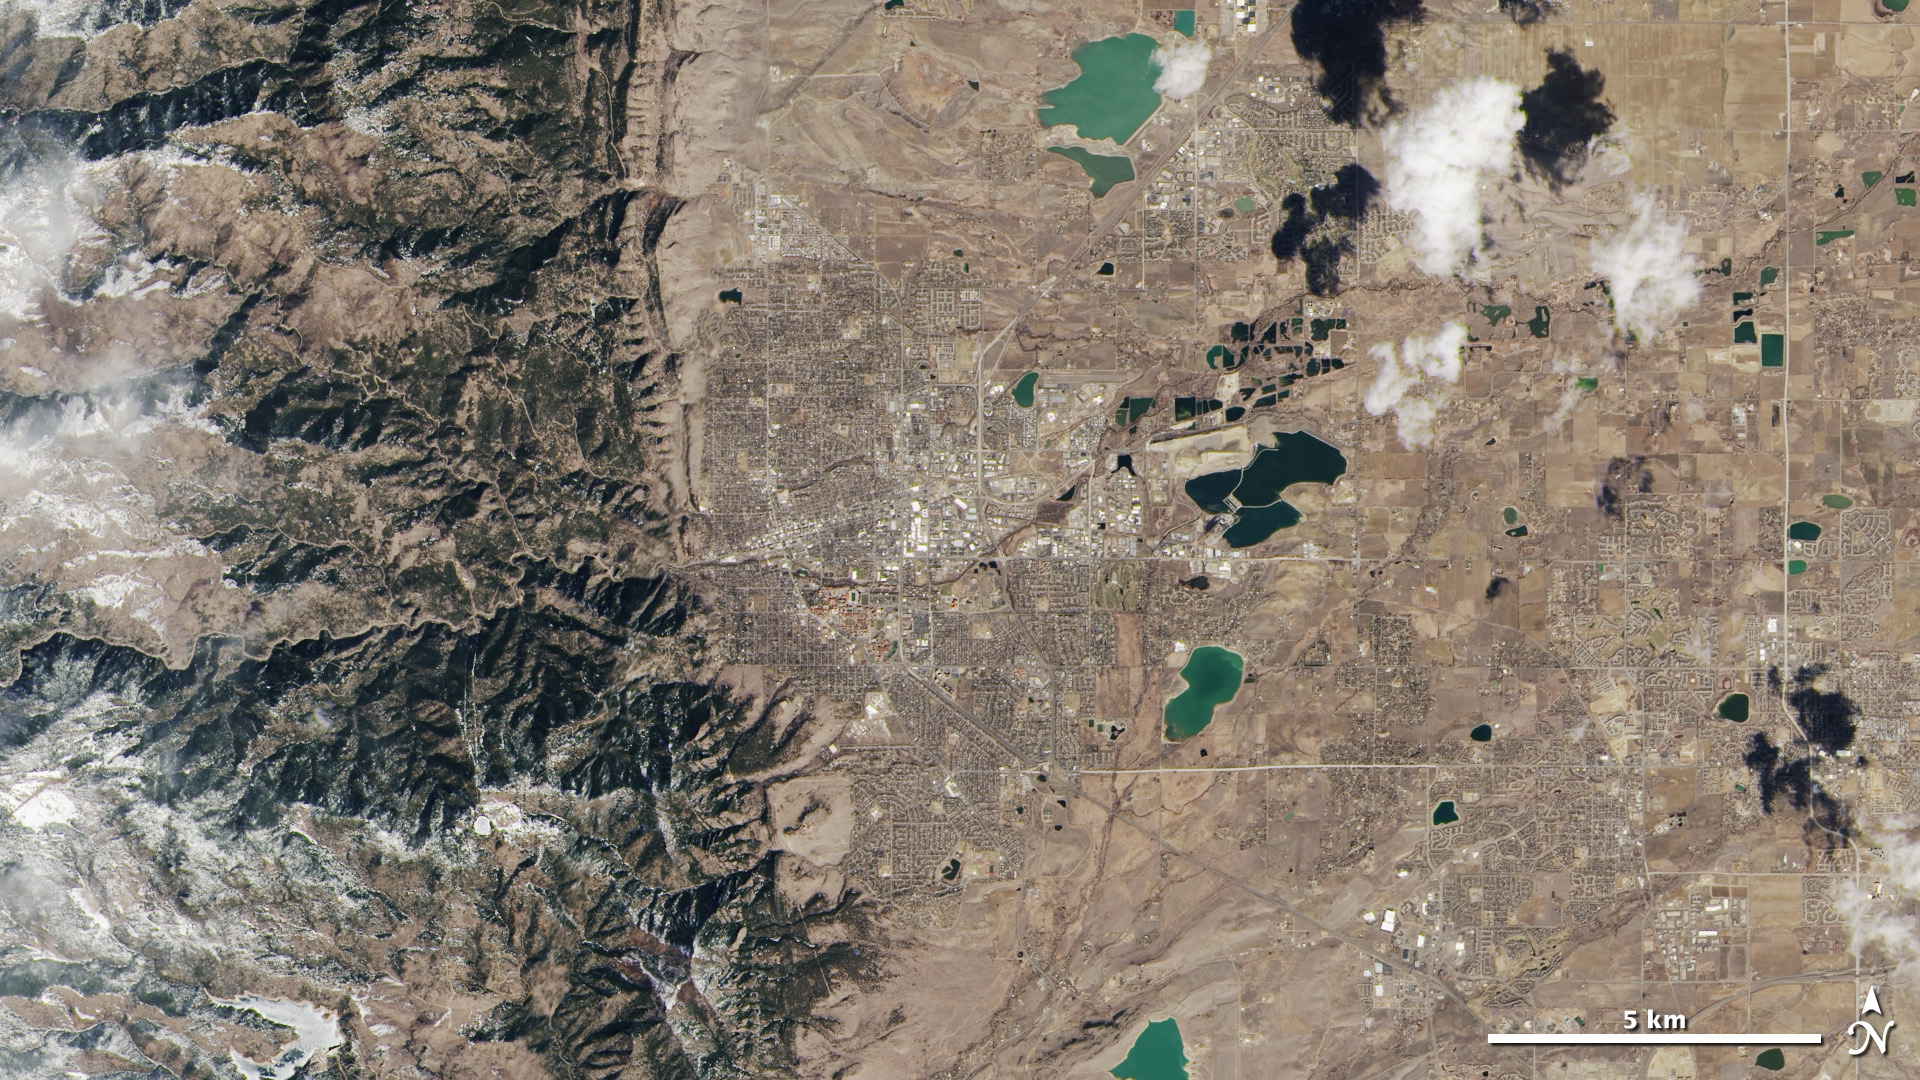
\includegraphics[width=\textwidth]{C:/Users/thiago/OneDrive/UNESP/Pos_graduacao/Eco/2015/Estatistica_2015/Aulas/Aula_1_Intro_2015/figs/landsat8.jpg}

\end{frame}
%===============================================================================%


%===============================================================================%
\begin{frame}
\centering
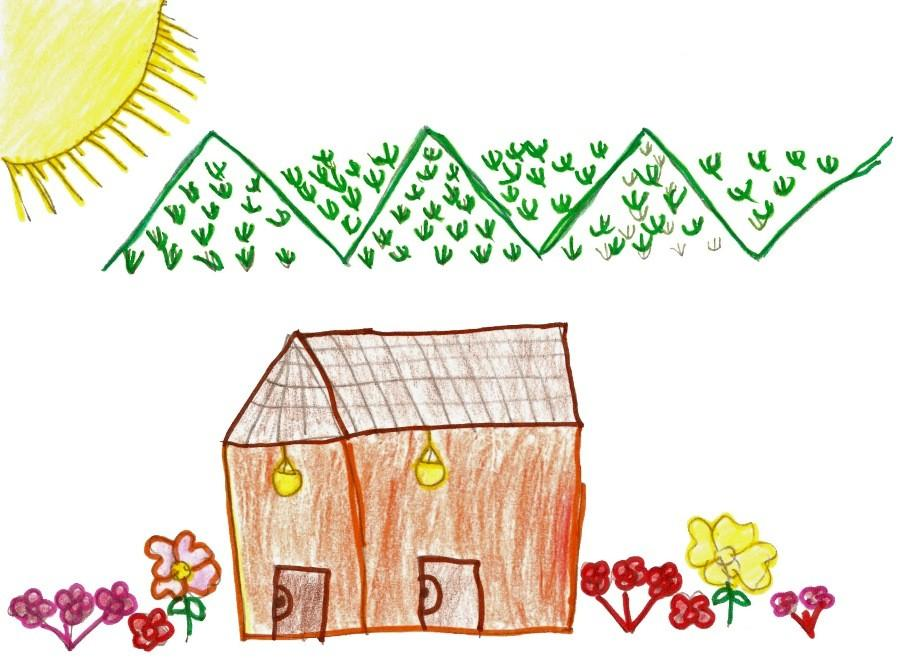
\includegraphics[width=\textwidth]{C:/Users/thiago/OneDrive/UNESP/Pos_graduacao/Eco/2015/Estatistica_2015/Aulas/Aula_1_Intro_2015/figs/casa.jpg}
\end{frame}
%===============================================================================%



%===============================================================================%
\begin{frame}{O que é um modelo?}
  \begin{itemize}
		\item
			Uma representação \textbf{simplificada} da realidade
      
      \vfill
		\item
			Busca descrever alguns aspectos de interesse, ignorando outros
	\end{itemize}


\vfill

\alert{\textbf{``All models are wrong. Some are useful'' - George E. P. Box}}

\end{frame}
%===============================================================================%




%===============================================================================%
\begin{frame}[t]
    \frametitle{Uma taxonomia de modelos}
    \begin{tikzpicture}
    \only<1>{\Tree [.Modelos Conceituais Quantitativos ]}
    \only<2>{\Tree [.Modelos \alert{Conceituais} [.Quantitativos Matemáticos Estatísticos ]]}
    \only<3>{\Tree [.Modelos \alert{Conceituais} [.Quantitativos [.Matemáticos Determinísticos ] [.Estatísticos Estocásticos ]]]}
    \only<4-5>{\Tree [.Modelos \alert{Conceituais} [.Quantitativos [.Matemáticos [.Determinísticos Teóricos ]] [.Estatísticos [.Estocásticos Empíricos ]]]]}
		    \end{tikzpicture}

\vfill

\only<5> {\textbf{Atenção: Essas relações \emph{não} são obrigatórias!}}

\end{frame}
%===============================================================================%

\section{Probabilidade}

%===============================================================================%
\begin{frame}{Probabilidade}

 \begin{itemize}
   \item A base de toda a estatística
    \vfill
   \item Conceitualmente simples\ldots
    \vfill
   \item \ldots mas que rapidamente se torna \textbf{bem complexa}.
    \vfill
   \item A probabilidade mede as ``chances'' de um determinado evento ocorrer
 \end{itemize}
 \vfill
\emph{Ex.: Qual a probabilidade de um inseto ser capturado por uma planta carnívora?}

\end{frame} 
%===============================================================================% 


%===============================================================================
\begin{frame}{Probabilidade}

Para falar de probabilidade, precisamos definir alguns termos:

\begin{itemize}
  \item \textbf{Evento ($A$):} um processo probabilístico (Ex.: $A$ = tentativa de captura) \pause
  \vfill
  \item \textbf{Resultado (\emph{outcome, $A_i$}): }resultado observado do evento (Ex.: $A_1$ = hove captura) \pause
  \vfill
  \item \textbf{Espaço (Universo) Amostral ($S = A_i,...,A_n$):} todos os resultados possíveis de um evento (Ex: $S_{captura} =$ \{Houve Captura, Não Houve Captura\}) \pause
  \vfill
    \item Neste exemplo, o espaço amostral é discreto
    
\end{itemize}


\end{frame} 
%===============================================================================%


%===============================================================================
\begin{frame}{Probabilidade em 15 minutos}

\textbf{Axioma 1:}
A probabilidade de qualquer evento dentro do espaço amostral é um número real positivo
\begin{equation*}
    P(A) \in \mathbb{R}, P(A) \geq 0  \quad \forall A \in S
\end{equation*}

\textbf{Axioma 2:}
A soma das probabilidades de todos os resultados dentro do espaço amostral é igual a 1
\begin{equation*}
    \sum_{i=1}^{n}{P(A_i)= 1}
\end{equation*}

\end{frame} 
%===============================================================================%


%===============================================================================
\begin{frame}{Probabilidade em 15 minutos}

\textbf{Regra da Subtração:} A probabilidade de observar um determinado resultado é complementar à probabilidade deste resultado não ser observado


\begin{equation*}
    P(A) = 1 - P(A^c) 
\end{equation*}

\alert{Ex.:} Qual a probabilidade de tirarmos 5 em um dado?


\begin{equation*}
    P(A) = \frac{1}{6} = 1 - P(A^c) = 1 - \frac{5}{6} = \frac{1}{6}
\end{equation*}



\end{frame} 
%===============================================================================%


%===============================================================================
\begin{frame}{Probabilidade em 15 minutos}

\textbf{Regra da Multiplicação:} Se dois eventos são \textbf{independentes}, a probabilidade de que os dois ocorram juntos é o \texbf{produto} da probabilidade de cada evento (\textbf{interseção das probabilidades}, $\cap$)
\begin{equation*}
    P(A \cap B) = P(A) \times P(B)
\end{equation*}

\alert{Ex.:} Qual a probabilidade de tirarmos um 5 \textbf{\emph{e}} um 6 em dois dados?


\begin{equation*}
    P(A \cap B) = P(A) \times P(B) = \frac{1}{6} \times \frac{1}{6} = \frac{1}{36}
\end{equation*}



\end{frame} 
%===============================================================================%


%===============================================================================
\begin{frame}{Probabilidade em 15 minutos}

\textbf{Regra da Adição:} Se dois eventos são \textbf{mutuamente exclusivos (disjuntos)}, a probabilidade de que algum deles ocorra é a \texbf{soma} da probabilidade de cada evento (\textbf{união das probabilidades}, $\cup$)
\begin{equation*}
    P(A \cup B) = P(A) + P(B)
\end{equation*}

\alert{Ex.:} Qual a probabilidade de tirarmos um 5 \textbf{\emph{ou}} um 6 em um dado?


\begin{equation*}
    P(A \cup B) = P(A) + P(B) = \frac{1}{6} + \frac{1}{6} = \frac{2}{6}
\end{equation*}



\end{frame} 
%===============================================================================%

%===============================================================================
\begin{frame}{Probabilidade em 15 minutos}

Se dois eventos \textbf{não} são mutuamente exclusivos, usamos: $P(A \cup B) = P(A) + P(B) - P(A \cap B)

\alert{Ex.:} Qual a probabilidade de sortearmos um 7 ($A$) \textbf{ou} uma carta de espadas ($B$) de um baralho com 52 cartas?

\begin{equation*}
    P(A=7)= \frac{4}{52} = 0.077, P(B = \text{espadas}) = \frac{13}{52} = 0.25
\end{equation*}

\begin{equation*}
    P(A \cup B) = P(A) + P(B) - P(A \cap B) = 0.077 + 0.25 - (0.077 \times 0.25) = 0.308
\end{equation*}

\center{\textbf{Por que subtrair $P(A \cap B)$?}}

\end{frame} 
%===============================================================================%


%===============================================================================
\begin{frame}{Probabilidade em 15 minutos}

\begin{small}

\textbf{Probabilidade condicional:} é a probabilidade de que um evento ocorra, dado que outro evento relacionado \textbf{já ocorreu}:

$P(A|B) = P(A \cap B)/P(B)$

\alert{Ex.:} Qual a probabilidade de uma carta sorteada ser um 7 ($A$), sabendo que a carta é de espadas ($B$)? 

\begin{equation*}
    P(A=7)= \frac{4}{52} = 0.077, P(B = \text{espadas}) = \frac{13}{52} = 0.25
\end{equation*}

\begin{equation*}
    P(A|B) = \frac{P(A \cap B)}{P(B)} = \frac{0.077 \times 0.25}{0.25} = 0.077
\end{equation*}

\center{\textbf{Se já sabemos que a carta é de espadas, a probabilidade de obter um 7 é 1/13, que equivale a 4/52}}

\end{small}

\end{frame} 
%===============================================================================%



%===============================================================================
\begin{frame}{Probabilidade em 15 minutos}

\textbf{Multiplicação para eventos dependentes:} Se dois eventos são \textbf{dependentes}, a probabilidade de que os dois ocorram juntos pode ser obtida pela relação anterior: 

\begin{equation*}
    P(A|B) = \frac{P(A \cap B)}{P(B)},  \quad P(A \cap B) = P(B) \times P(A|B)
\end{equation*}

\alert{Ex.:} Em Rio Claro, a chance de ser picado por \emph{Aedes egyptii} ($C$) é de 70\% por dia. Assumindo que a chance de um mosquito transmitir o vírus ($T$) é de 50\% , qual a probabilidade de um aluno de estatística pegar dengue hoje?



\end{frame} 
%===============================================================================%


%===============================================================================
\begin{frame}{Probabilidade em 15 minutos}

A probabilida de transmissão é condicional à picada. Se houve picada, $P(A | B) = 0.5$. Se não houve picada, $P(A | B) = 0$.

 
 \begin{equation*}
     P(A \cap B) = P(B) \times P(A | B) 
 \end{equation*}
 
  \begin{equation*}
     P(T \cap C) = P(C) \times P(T | C) = 0.7 \times 0.5 = 0.35
 \end{equation*}
 

\end{frame} 
%===============================================================================%

%===============================================================================
\begin{frame}{Exercício: Gotellli \& Ellison 2$^a$ Ed. Ing. pp. 15-17}

\textbf{Plantas vs. lagartas}

\begin{small}

Em uma paisagem, temos manchas de dois fenótipos de uma planta: $R$ é resistente à herbivoria por lagartas, enquanto $R^c$ não é. Os fenótipos nunca ocorrem juntos na mesma mancha, e fenótipos resistentes ocorrem na paisagem com frequência  de 20$\%$.

A probabilidade de uma mancha ser invadida por lagartas ($C$) é de 0.7, independente da variedade.
\vfill

Assumindo que as lagartas se dispersam igualmente para todas as manchas, e que somente populações resistentes sobrevivem à chegada das lagartas, qual a probabilidade de que uma mancha desapareça devido à herbivoria? 
\vfill
\alert{\textbf{Dica:}} Primeiro calcule as probabilidades de ocorrência das quatro combinações possíveis de resultados.

\end{small}

\end{frame}
%===============================================================================%

%===============================================================================
\begin{frame}{Exercício: Gotellli \& Ellison 2$^a$ Ed. Ing. pp. 15-17}

\textbf{Primeiro Passo:} organizando as informações:
\vfill
\tqt{Resistente} ou \tqt{suscetível} são resultados mutuamente exclusivos:

$P(R) = 0.2, \quad P(R^c) = P(1 - R) = 0.8$
\vfill
Presença e ausência de lagartas são resultados mutuamente exclusivos:

$P(L) = 0.7, \quad P(L^c) = P(1 - L) = 0.3$

\vfill
$S = \{R^cL^c,RL^c,RL,R^cL,RL\}$

\end{frame}
%===============================================================================%


%===============================================================================
\begin{frame}{Exercício: Gotellli & Ellison 2nd Ed. Ing. pp. 15-17}

\textbf{Segundo Passo:} Expressando as probabilidades. Resistência e invasão por lagartas são eventos independentes:

\vfill
$P(R^cL^c) = P(R^c) \times P(L^c)$
\vfill
$P(RL^c) = P(R) \times P(L^c)$
\vfill
$P(R^cL) = P(R^c) \times P(L)$
\vfill
$P(RL) = P(R) \times P(L)$
\vfill
Multiplicamos porque os eventos são independentes.

\end{frame}
%===============================================================================%

%===============================================================================
\begin{frame}{Exercício: Gotellli \& Ellison 2$^a$ Ed. Ing. pp. 15-17}

\textbf{Terceiro Passo:} Calculando as probabilidades:
\vfill
$P(R^c \cap L^c) = P(R^c) \times P(L^c) = 0.8 \times 0.3 = 0.24$
\vfill
$P(R \cap L^c) = P(R) \times P(L^c) = 0.2 \times 0.3 = 0.06$
\vfill
$P(R^c \cap L) = P(R^c) \times P(L) = 0.8 \times 0.7 = 0.56$
\vfill
$P(R \cap L) = P(R) \times P(L) = 0.2 \times 0.7 = 0.14$


\end{frame}
%===============================================================================%

%===============================================================================
\begin{frame}{Exercício: Gotellli \& Ellison 2$^a$ Ed. Ing. pp. 15-17}
\textbf{Quarto Passo:} Combinando as probabilidades:
\begin{small}
\vfill
$P(R^c \cap L^c) = P(R^c) \times P(L^c) = 0.8 \times 0.3 = 0.24$ : Planta permanece
\vfill
$P(R \cap L^c) = P(R) \times P(L^c) = 0.2 \times 0.3 = 0.06$ : Planta permanece
\vfill
$P(R^c \cap L) = P(R^c) \times P(L) = 0.8 \times 0.7 = 0.56$ : \textbf{Planta desaparece}
\vfill
$P(R \cap L) = P(R) \times P(L) = 0.2 \times 0.7 = 0.14$ : Planta permanece
\vfill
\end{small}
$\mathbf{P(\textbf{Planta desaparece}) = 0.56}$

$P(\text{Planta permanece}) = P((R^c \cap L^c) \cup (R \cap L^c) \cup (R \cap L))  = 0.44$ 

\end{frame}
%===============================================================================%



%===============================================================================
\begin{frame}{Expandindo o Exercício}

\textbf{Plantas vs. lagartas vs. invasoras}

\begin{small}

Mesmo nos fenótipos resistentes, a herbivoria diminui a capacidade competitiva da planta estudada, facilitando o estabelecimento ($I$) de uma espécie invasora. Se há presença da lagarta, a invasão tem uma taxa de sucesso de 60\%, e se não há plantas, o sucesso é garantido (100\%). 
\vfill
Qual a probilidade de que haja invasão, sabendo que as lagartas já atingiram a mancha?

\end{small}

\end{frame}
%===============================================================================%

%===============================================================================
\begin{frame}{Expandindo o Exercício}

\begin{small}

O primeiro impulso é calcular $P(I \cap L) = P(I|L) \times P(L)$. Mas a herbivoria leva à remoção da planta quando esta não é resistente, modificando a probabilidade de invasão.

Temos, assim, duas probabilidades condicionais:

$P(I \cap R^cL) = P(I|R^cL) \times P(R^cL) = 1 \times 0.56 = 0.56$
\vfill
$P(I \cap RL) = P(I|RL) \times P(RL) = 0.6 \times 0.14 = 0.084$
\vfill
$RL$ e $R^cL$ são mutuamente exclusivos, então temos:

$P(I \cap L) = P(I \cap R^cL) \cup P(I \cap RL) = 0.56 + 0.084  = 0.644$


\end{small}

\end{frame}
%===============================================================================%


%===============================================================================
\begin{frame}{Estimando Probabilidades}

\emph{Qual a probabilidade de uma planta carnívora capturar um inseto?}

\begin{itemize}
  \item \textbf{Como podemos estimar essa probabilidade?} \pause
  \vfill
  \item Realizando uma \textbf{contagem} dos sucessos e fracassos da planta, para várias visitas de insetos.\pause
  \vfill
  \item Cada visita individual é uma \textbf{realização} do evento: capturado ou não. Também conhecida como \textbf{réplica} ou \textbf{observação}.\pause
  \vfill
  \item O conjunto de realizações sucessivas compreende um \textbf{experimento}.
\end{itemize}

\end{frame} 
%===============================================================================%


%===============================================================================
\begin{frame}{Frequência vs. Probabilidade}

\begin{centering}

\textbf{Frequência de Captura:}

\begin{equation*}
    F  = \frac{\text{número de capturas}}{\text{número de visitas}}
\end{equation*}


\end{centering}

\end{frame} 
%===============================================================================%


%===============================================================================
\begin{frame}{Frequência vs. Probabilidade}

\begin{centering}

\textbf{Frequência de Captura:}

\begin{equation*}
    F = \frac{\text{número de sucessos}}{\text{número de realizações}}
\end{equation*}


\end{centering}

\end{frame} 
%===============================================================================%


%===============================================================================
\begin{frame}{Frequência vs. Probabilidade}

\begin{centering}

\textbf{Probabilidade de Captura:}

\begin{equation*}
    P(\text{captura}) \approx \lim_{n_t \to \infty} \frac{\text{número de sucessos} (n_r)}{\text{número de realizações } (n_t)}
\end{equation*}

\end{centering}

\end{frame} 
%===============================================================================%

%===============================================================================%
\begin{frame}{Culturas Estatísticas}

\textbf{Estatística Frequentista:}

\begin{itemize}

  \item Associada principalmente a \emph{Sir} Ronald Aymer Fisher, FRS.
\vfill
  \item Se baseia na associação entre frequências e probabilidades.
\vfill
  \item Ex: Jogo uma moeda 100 vezes, obtenho 45 caras e 55 coroas. Estimo minhas probabilidades como 0.45 e 0.55
\vfill
  \item Vê a amostra como uma realização aleatória de um evento
\vfill
  \item Parte do princípio de que se o processo fosse repetido infinitamente, seria possivel estimar as probabilidades associadas aos resultados do evento
  
\end{itemize}
 
\end{frame}
%===============================================================================%


%===============================================================================%
\begin{frame}{Culturas Estatísticas}

\begin{centering}

  $p < 0.05$? \pause
\vfill
  $P(A|H)$ ou $P(H|A)$? \pause
\vfill
  É a mesma coisa?

\end{centering}
 
\end{frame}
%===============================================================================%



%===============================================================================%
\begin{frame}{Culturas Estatísticas}

\begin{small}

Na visão frequentista, se avalia a probabilidade de se obter a amostra observada, dada uma determinada hipótese:

\begin{equation*}
P(A|H)
\end{equation*}

\alert{Ex:} Joguei uma moeda 100 vezes, e obtive 65 caras e 35 coroas. Se a minha hipótese é de que a moeda é honesta ($P(\text{cara}) = P(\text{coroa}) = 0.5$), qual chance de eu obter esse resultado, \textbf{ou um resultado mais extremo}?

\begin{equation*}
p =\ensuremath{8.6\times 10^{-4}}
\end{equation*}

Se eu repetir esse experimento infinitas vezes (jogar 100 moedas), vou encontrar um resultado igual ou mais extremo 0.086\% das vezes.

\end{small} 
 
\end{frame}
%===============================================================================%

%===============================================================================%
\begin{frame}{Culturas Estatísticas}

A lógica nos diz que o mais importante é saber $P(H|S)$. Mas como? \pause

\centering{\textbf{Teorema de Bayes:}}

\begin{equation*}
P(H \mid A) = \frac{P(H \cap A)}{P(A)} =\frac{P(A \mid H) \times P(H)}{P(A)}
\end{equation*}

$P(A | H)$: probabilidade da amostra se a hipótese é verdadeira

$P(A)$: probabilidade da amostra, garante que $0 \leq P(H | A)$ \leq 1$

$\mathbf{P(H)}$: probabilidade da hipótese ser verdadeira. Conhecida como \textbf{priori (prior)}.



\end{frame}
%===============================================================================%

%===============================================================================%
\begin{frame}{Culturas Estatísticas}

\textbf{Estatística Bayesiana}

\begin{itemize}

  \item Associada a Thomas Bayes

 \item Na visão bayesiana, a análise estatística serve para \texbf{atualizar} o conhecimento anterior

 \item O conhecimento prévio pode ser usado para definir uma probabilidade \emph{priori} da hipótese ser verdadeira 
 
 \item O resultado do experimento permite que voce atualize (melhore) essa estimativa de probabilidade, com base na amostra observada.

\end{itemize}

\end{frame}
%===============================================================================%


%===============================================================================%
\begin{frame}{Estatística Bayesiana}

\alert{Ex.:} Joguei uma moeda 100 vezes, e obtive 65 caras e 35 coroas. Se a minha hipótese é de que a moeda é honesta ($P(\text{cara}) = P(\text{coroa}) = 0.5$), qual a probabilidade que essa hipótese esteja correta?
\vfill

$H_0$: A moeda é honesta

$H_1$: A moeda é tendenciosa

\vfill
Baseado em meu conhecimento de moedas, eu poderia dizer que a probabilidade dela ser honesta é 0.9 ($P(H_0) = 0.9$), e a probabilidade dela ser tendenciosa é 0.1 ($P(H_1) = 0.1$). 
 
\end{frame}
%===============================================================================%

%===============================================================================%
\begin{frame}{Estatística Bayesiana}

Para H$_0$:

\begin{equation*}
P(H_0|A) = \frac{P(A|H_0) \times P(H_0)}{P(A)}
\end{equation*}

\begin{equation*}
P(H_0 | A) = \frac{P(A | H_0) \times P(H_0)}{P(A | H_0) \times P(H_0) + P(A | H_1) \times P(H_1)}
\end{equation*}

\begin{equation*}
P(H_0 | A) = \frac{P(\ensuremath{8.6\times 10^{-4}})P(0.9)}{\ensuremath{8.6\times 10^{-4}}\times 0.9 +0.0834 \times 0.1}
\end{equation*}

$P(H_0|A) = 0.085$
 
\end{frame}
%===============================================================================%

%===============================================================================%
\begin{frame}{Estatística Bayesiana}

Para H$_1$:

\begin{equation*}
P(H_1 | A) = \frac{P(A | H_1) \times P(H_1)}{P(A)}
\end{equation*}

\begin{equation*}
P(H_1 | A) = \frac{P(A | H_1) \times P(H_1)}{P(A | H_1) \times P(H_1) + P(A | H_0) \times P(H_0)}
\end{equation*}

\begin{equation*}
P(H_0 | A) = \frac{P(0.0834) \times P(0.1)}{0.0834 \times 0.1 +\ensuremath{8.6\times 10^{-4}} \times 0.9}
\end{equation*}

$P(H_1|A) = 0.915$
 
\end{frame}
%===============================================================================%



%===============================================================================%
\begin{frame}{Estatística Bayesiana}

A escolha da \emph{priori} afeta fortememente a \emph{posteriori}:
\vfill

\begin{small}

$\mathbf{P(H_0=0.5),P(H_1=0.5)} \rightarrow P(H_0|S) = 0.01, P(H_1|S) = 0.98$

\vfill

$\mathbf{P(H_0=0.75),P(H_1=0.25)} \rightarrow P(H_0|S) = 0.03 , P(H_1|S) = 0.97$

\vfill

$\mathbf{P(H_0=0.95),P(H_1=0.05)} \rightarrow P(H_0|S) = 0.16, P(H_1|S) = 0.84$

\vfill

$\mathbf{P(H_0=0.99),P(H_1=0.01)} \rightarrow P(H_0S) = 0.506, P(H_1|S) = 0.494$

\end{small}

\end{frame}
%===============================================================================%

%===============================================================================%
\begin{frame}{Frequentista vs. Bayesiana}

\begin{columns}[lr]

\column{.5\textwidth}

\begin{scriptsize}
\textbf{Bayesianos sobre frequentistas:
}
\begin{itemize}

  \item{Ignoram qualquer informação a priori}
  
  \item{Se baseiam em experimentos fictícios}
  
\end{itemize}

\vspace{.5in}

\textbf{Frequentistas sobre Bayesianos:}

\begin{itemize}

  \item{Podem gerar o resultado que quiserem manipulando as \emph{priori}}
  
\end{itemize}

\end{scriptsize}

\column{.5\textwidth}

  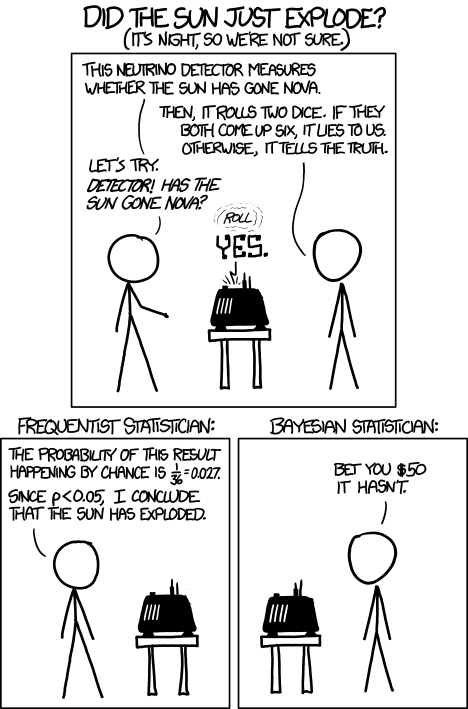
\includegraphics[width=2in]{C:/Users/thiago/OneDrive/UNESP/Pos_graduacao/Eco/2015/Estatistica_2015/Aulas/Aula_1_Intro_2015/figs/frequentists_vs_bayesians.png}
  \tiny{\center{http://xkcd.com/1132/}}

\end{columns}


\end{frame}
%===============================================================================%


%===============================================================================%
\begin{frame}{Qual vamos usar?}

\textbf{O Curso se baseará na filosofia frequentista.}

\begin{itemize}

\item Mais frequentemente usada (\emph{tu-dum psh}).

\item Mais familiar à comunidade ecológico-científica.

\item É a estatística com a qual voces já tiveram algum contato prévio.

\item É a que eu sei ensinar.

\end{itemize}

\textbf{Contudo, tomaremos cuidado em enfatizar os maus usos e compreensões equivocadas da estatística frequentista.}
  
  
\end{frame}
%===============================================================================%

%===============================================================================%
\begin{frame}[t]{Por que usar R?}

\begin{columns}[t]

\column{2.5in}
\begin{footnotesize}

\textbf{R:} Software para análise e programação estatística - \textbf{Uso obrigatório no curso}. 

\begin{itemize}

	\item Livre, gratuito, tem se tornado ``padrão'' para análise de dados
      
  \item	Difícil no início, mas o tempo é recuperado depois
    
	\item	Programação =  liberdade 
	
  \item Todos os exercícios do curso devem ser feitos em R
		
  \item	Assume-se que todos tenham instalado o R 3.1.3 e a interface RStudio.
	
  \end{itemize}
	
  \end{footnotesize}
  
\column{1.5in}
	
	\centering
	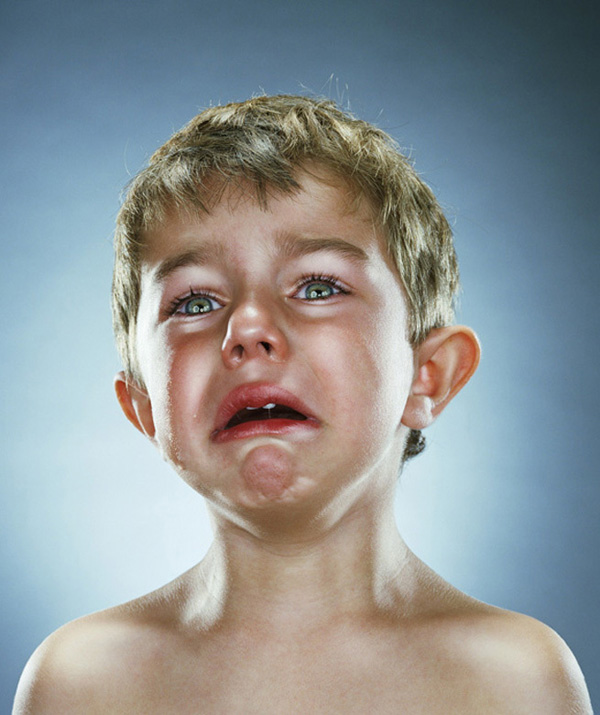
\includegraphics[width=1.5in]{C:/Users/thiago/OneDrive/UNESP/Pos_graduacao/Eco/2015/Estatistica_2015/Aulas/Aula_1_Intro_2015/figs/crybaby.jpg}
	
	\tiny{http://www.jillgreenberg.com/}
	
\end{columns}
	
\end{frame}
%===============================================================================%


% %===============================================================================%
% \begin{frame}{Para a tarde}
% 
% \textbf{Leitura e discussão:}
% 
% \vfill
% 
% \begin{itemize}
% 
% \item Martínez-Abraín A (2007) Are there any differences? A non-sensical question in ecology. Acta Oecologica, 32, 203–206.
% 
% \vfill
% 
% \item Gigerenzer G (2004) Mindless statistics. The Journal of Socio-Economics, 33, 587–606.
% 
% \end{itemize}
%   
% \center{(Artigos no Dropbox)}
%   
% \end{frame}
% %===============================================================================%



%===============================================================================%
%===============================================================================%
\end{document}
%===============================================================================%
%===============================================================================%
